% !TEX root = arbeit.tex
\section{Theory}

	\subsection{Requirements}
	% Mass, performance, Power consumption. (See latest references)
	
	\subsection{Basic Theory about a TOF instrument}
	A time of flight mass spectrometer consists of, an ion-source, a mass analyser and a detector.\\
	
	\begin{figure}[htb] % Noch schauen, ob das noch verschoben wird.
		\centering
		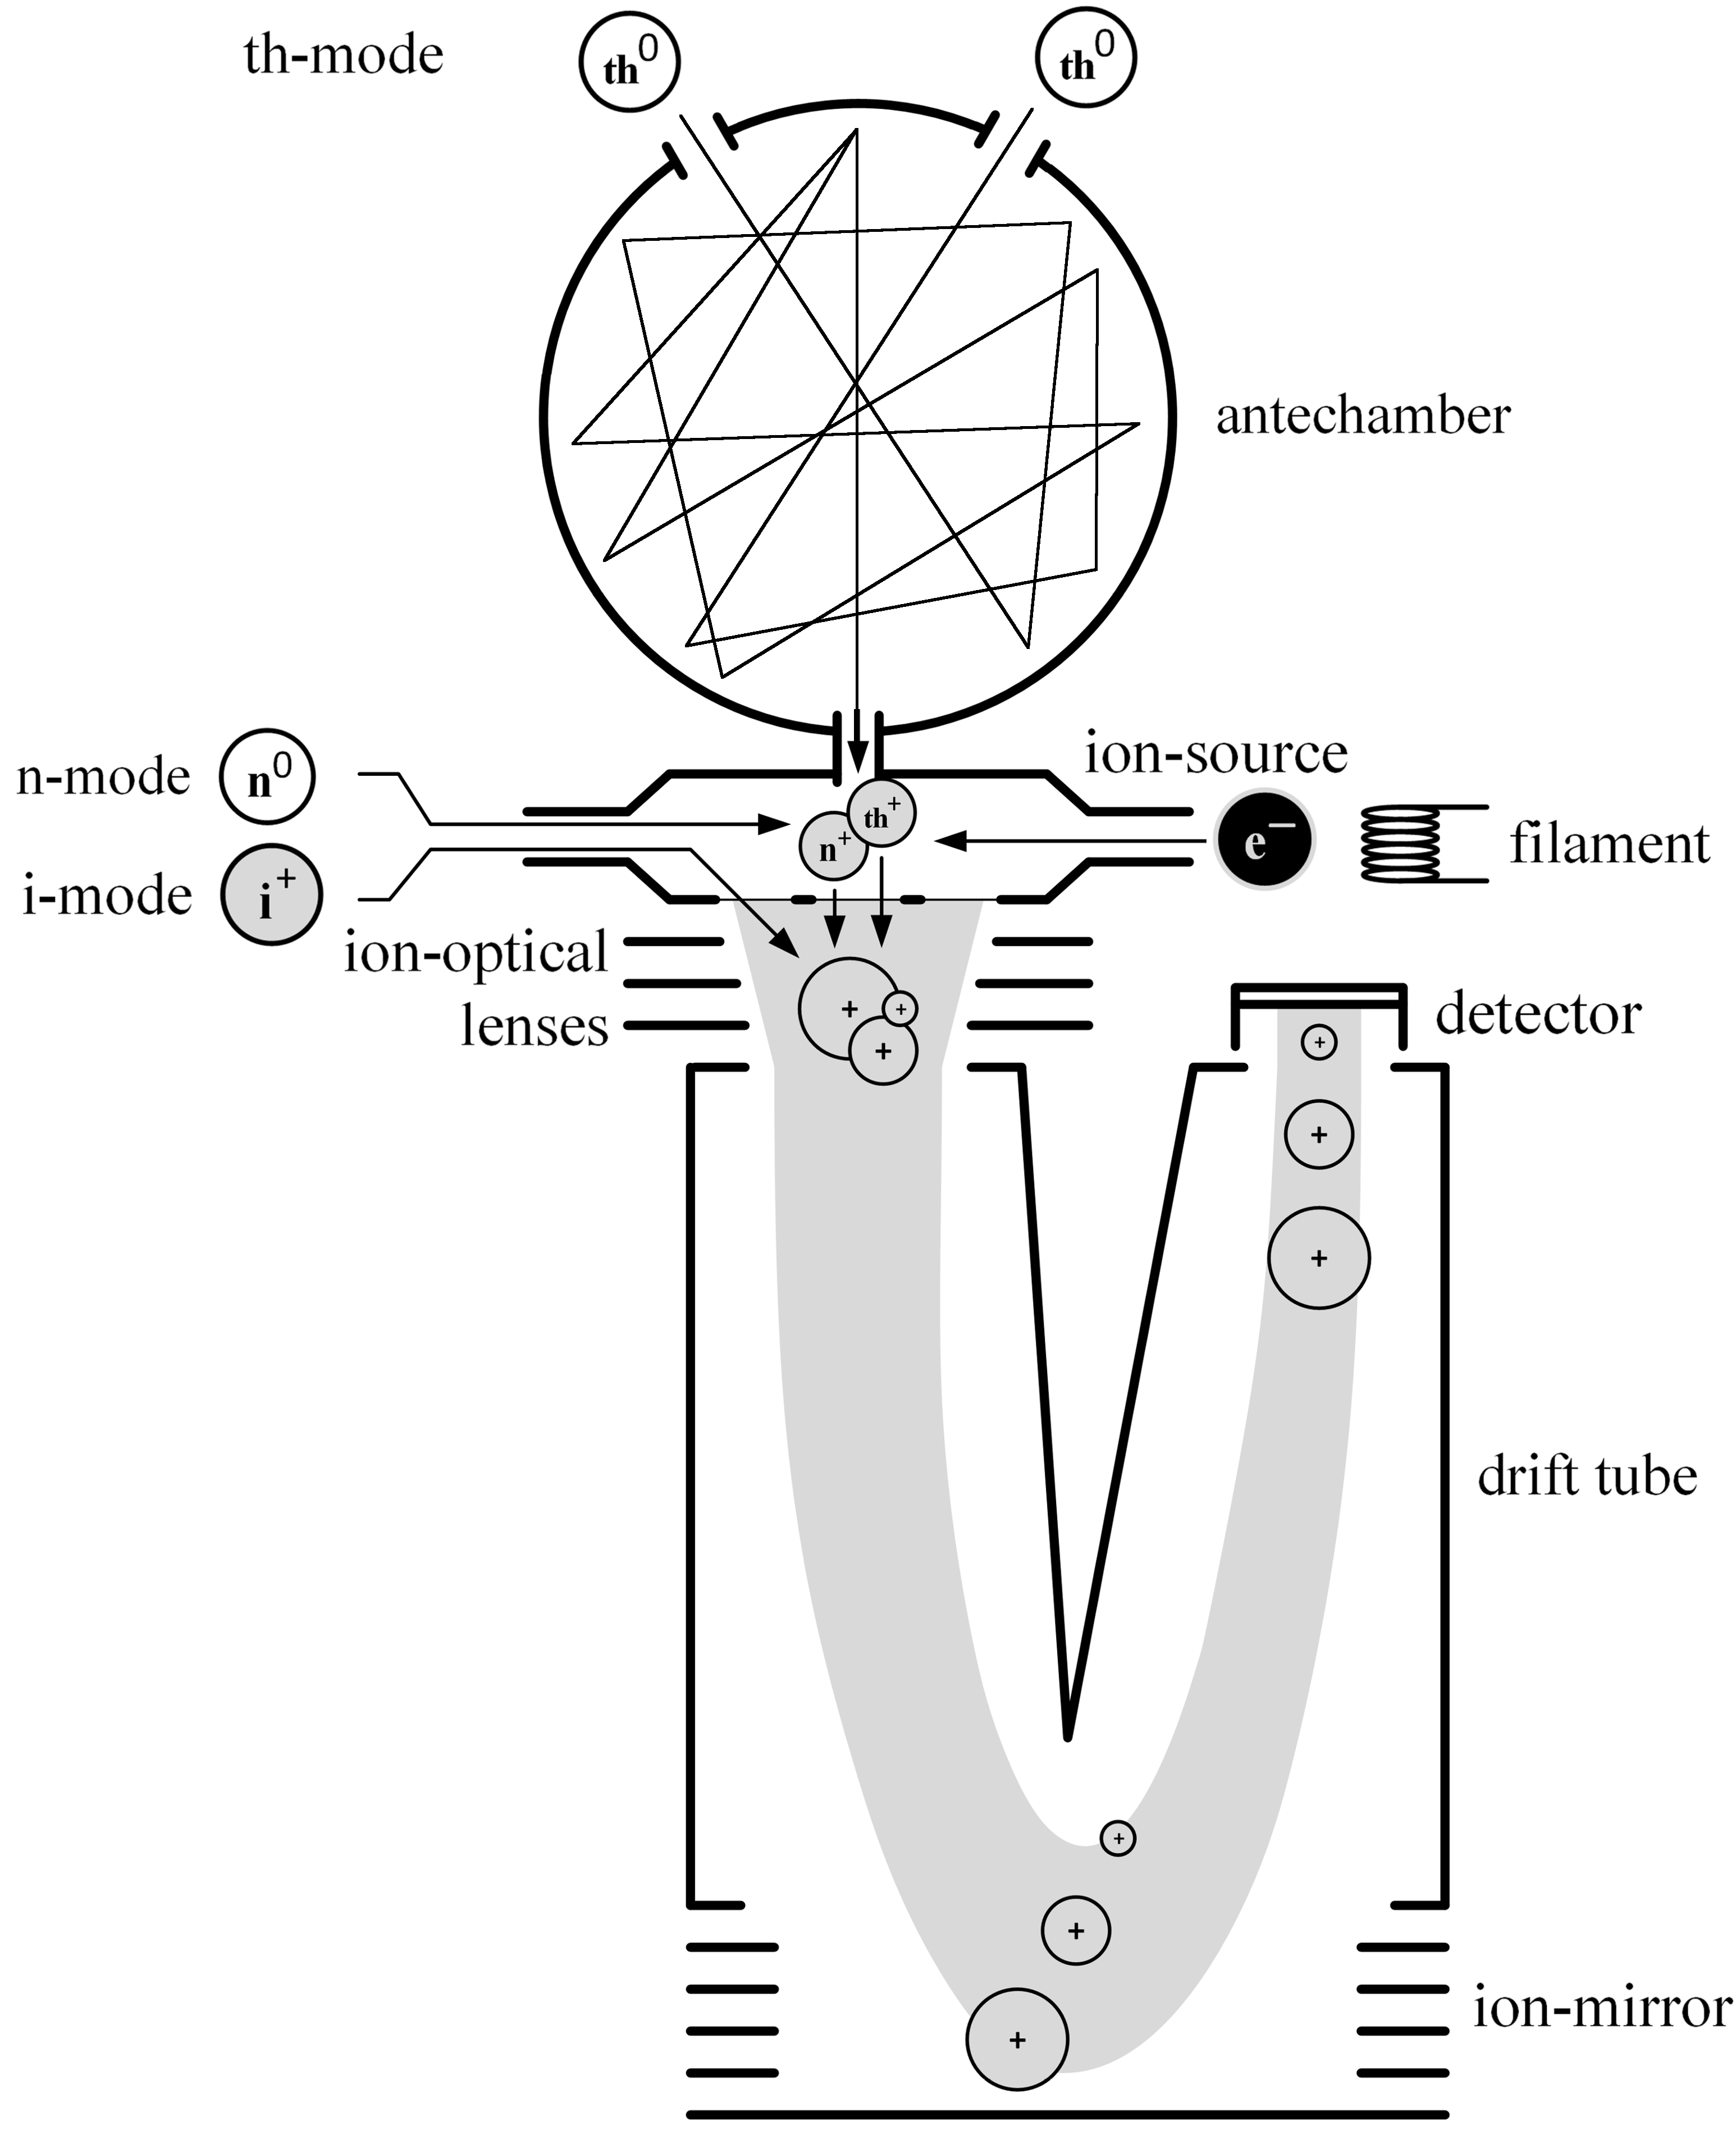
\includegraphics[width= 10cm]{Bilder/NIM_Sketch.png} % Bei Bild noch schauen, ob die Ränder drauf sind. Bei Zeiten noch Bild anpassen.
		\caption{Schematics of the NIM mass spectrometer. Adapted from \cite{Diss_Meyer}.}
		\label{fig:NIMSketch}
	\end{figure}

	%First overview and then go into the details.
	In the ion-source, the ions are formed. The NIM instrument is able to measure neutrals and ions. Ions entering the source are let directly to the mass analyser. Neutral particles get ionised with and electron emitting filament. % Noch genaue Formulierung nachschauen.
	The formed ions get accelerated to the same energy and fly through the spectrometer. Light particles fly faster through the spectrometer than heavier ones. The different particle species arrive at different times at the detector. The used detector is an MCP detector. To enhance the flight distance without enlarge the instrument, an ion-mirror is used.
	
		\subsubsection{Ion-source}
		To calculate the number of ions produced in the ion source we use:
		\begin{equation}
		I_{ion} = \beta\cdot Q_{ion}\cdot L\cdot n\cdot I_{em}
		\end{equation}
		With $\beta$ the extraction efficiency which is 1, % Noch schauen auf welchen Wert wir diese setzen wollen. 1= sehr gute Quelle, 0.01 = 1mus/100mus = Pulslänge Pulser/ Länge 1 Zyklus. Noch diskutieren, welche Werte beta haben kann oder einfach etwas setzen? Da die ersten Messresultate gut sind, würde ich eher auf 1 setzen.
		$L$ as the effective ionising path in our case 4~\si{\milli\metre}, $n$ the particle density, $I_{em}$ the electron emission current from the filament and $Q_{ion}$ the ionising cross section. The cross sections of species used in our calibration can be found in table % Ref. auf Tabelle und nur auf Stefans Diss verweisen oder die 4 Originalpaper zusammen suchen.
		
		% Reference: Bieler Diss 2012, Wurz 2011, Scherer 1999, Meyer 2013 Data Analysis, Wells 2011
		% Ionisation efficiency
		% Description of how it works with the energies. Electric -> kinetic. Pulser. E = 1/2 mv^2 = qU
		% Time focusing?
		% Mass calibration t/dt -> m/dm.
		% SNR definition. Picture?
		% Sensitivity estimation. Nessesary? If so, part of SNR discussion.
		% MCP detector. Gain calculation.
		% Antchamber. Explanation of closed and open source. Field of view. Densitiy enhancement.
	
	
\begin{comment}
	
	Explain how a TOF works. Source, reflectron, detector.
	Explanation of the antechamber at the end after explaining the different parts.
	
	Detection efficiency Ionsource, MCP? -> y-Achse
	Mass Analyser, mass spectrometer. Most important formulas. dm/m = dt/t...
	Sensitivity
	Density enhancement -> explanation about closed and open source
	Sketch of the instrument
	Requirements: Power, mass, mass resolution,... (At the end or at the beginning)
	
	
	Ionisationseffizienz/ Ionenproduktion der wichtigsten Gase. Detektionseffizienz hängt auch von Effizienz der MCPs ab... Erklären weshalb man die Achsenskalieruing braucht (entweder Counts oder die angepasste a.u. bei der Fläche und Counts/s für das Spektrum)
	
\end{comment}
		